\chapter[Detecting chromatin accessibility as a mediator of gene expression in Collaborative Cross mice]{Detecting chromatin accessibility as a mediator of gene expression in Collaborative Cross mice
\footnote{This chapter was adapted from a portion of an early draft of a collaborative manuscript that is in preparation. Current author line and title are: Keele, G. R\textsuperscript{*}., Quach, B\textsuperscript{*}., Israel, J. W., Zhou, Y., Chappell, G. A., Lewis, L., Safi, A., Oreper D, Simon, J. M., Crawford, G. E., Valdar, W., Wright, F. A., Rusyn, I., Furey, T. S. Tissue-specific QTL analyses of gene expression and chromatin accessibility in the Collaborative Cross mouse population. Co-first authors\textsuperscript{*}.}}
\label{chap:mediation}

\section{Introduction}

Advancements in sequencing technologies over the last decade have made multi-omic experiments feasible, and further advancements in technology and interest are only increasing. Initially these data sets were observational, certainly due to the very real constraints of the populations (humans), the developing technology, and the challenge of coordinating very large experiments with multiple levels of data. With progress in these areas, powerful large-scale experiments with multiple dimensions of data per individual can be paired with modern statistical mediation analysis to draw inferences on the relationships that lie hidden between the levels of these data. These results will be more likely to identify causal rather than correlational elements, and thus provide more meaningful and actionable targets in terms of downstream applications in areas such as medicine and agriculture.

One area of strong interest has been the use of integrative analyses to better understand the regulation of fundamental biological processes that make up the processing of information from genomic DNA to phenotype, which has resulted in a variety of statistical approaches. \cite{Degner2012} noticed the co-localization of chromatin accessibility QTL (cQTL), assessed through DNAS I sequencing, and expression QTL (eQTL) in human lymphoblastoid cell lines, detecting correlations in their positions. \cite{Battle2014} investigated the regulation of gene expression in 922 humans, use eQTL and allele specific expression QTL. They did not measure chromatin accessibility, but assessed the evidence whether proximal genes to distal-eQTL behaved as mediators to the gene. \cite{Pai2015} did not use mediation, rather characterizing the location of eQTL in genomic regulatory elements in human lymphoblastoid cell line data. \cite{Alasoo2017} similarly did not use mediation with human cell lines, but rather further elucidated the roles of eQTL within regulatory elements through the use of bacterial infections to modify the enhancer primers. \cite{Roytman2018} used causal mediation models of histone modifications (hQTL) and expression (eQTL) to better detect signals in data from 112 humans. \cite{Wu2018} used mediation to tease apart the relationship of DNA methylation sites, gene expression, and complex traits. \cite{Battle2015} did not use mediation, but characterized the co-localization of QTL underlying gene expression (eQTL), ribosome occupancy (rQTL), and protein abundance (pQTL), detecting significant overlap as well as a buffering of QTL effect from ribosome occupancy up to protein abundance, again in human lymphoblastoid cell lines. \cite{Chick2016} used a genome-wide mediation approach to characterize the transcriptional and post-translational regulation of proteins in 192 Diversity Outbred (DO) mice \citep{Churchill2012}. These studies demonstrate the span and flexibility of integrative approaches.

One appealing feature of the DO is the potential to replicate results in its related inbred sister population, the Collaborative Cross (CC) \citep{Churchill2004,Hall2012,Srivastava2017}, a panel of recombinant inbred strains descended from the same founder inbred strains as the DO. \cite{Chick2016} take advantage of this and use CC mice to confirm results in the DO by showing that estimates of founder allele effects from each of the related populations corresponded. Similar to the DO, the CC represent a powerful untapped tool for these integrative analyses of multi-omic data. Though the CC possesses certain limitations in comparison to the DO, such as a restricted number of strains and thus unique genomes, and comparatively reduced mapping resolution, it also has strengths, mainly the potential for replicate observations, which are useful to reduce noise as well as valuable for potential downstream experiments. If the assumed additive model is true for the QTL, mapping is also more powerful in inbred animals in comparison to outbred ones.

In this work, we use a small sample of 47 male CC mice with single observation per strain to investigate the dynamics between chromatin accessibility and gene expression, as done in \cite{Degner2012} though here chromatin accessibility is measured through Assay for Transposase Accessible Chromatin sequencing (ATAC-Seq). To our knowledge, this is the first study of this kind in the CC. We aim to detect QTL underlying gene expression and chromatin accessibility separately in three tissues: lung, liver, and kidney. We will then assess the support for mediation of the effect of eQTL on gene expression through chromatin accessibility, using methods inspired by \citep{Chick2016}. We identify and characterize examples of strong mediation, as well as co-localizing but independent eQTL and cQTL. This study is an example of the experimental power of the CC for integrative analysis of multi-omic data, particularly given the limited sample size, and provides support for its continued use in larger, more complex experiments going forward.

\section{Materials and Methods}

\subsection{Animals}

Adult male mice (8-12 weeks old) from 47 CC strains were acquired from the University of North Carolina Systems Genetics Core (Chapel Hill, NC). Animals were maintained on an NTP 2000 wafer diet (Zeigler Brothers, Inc., Gardners, PA) and water \textit{ad libitum}. The housing room was maintained on a 12-h light-dark cycle. The experimental design sought to maximize the number of strains relative to within-strain replications based on the power analysis for QTL mapping in mouse populations \citep{Kaeppler1997}; therefore, one mouse was used per strain. Mice were euthanized between 8 and 10 a.m. and lungs, liver, and kidney tissues were collected, flash frozen in liquid nitrogen, and stored at -80\degree C until analysis. These studies were approved by the Institutional Animal Care and Use Committees at Texas A\&M University and the University of North Carolina.

\subsection{Collaborative Cross reference genomes and transcriptomes}

Sequencing read mapping required CC strain-specific reference genomes and transcriptomes denoted as ``pseudo-genomes" and ``pseudo-transcriptomes" respectively. Pseudo-genomes in FASTA file format and corresponding MOD files were downloaded from the CC resource website (\url{http://csbio.unc.edu/CCstatus/index.py?run=Pseudo}) for Build 37. The Build 37 MOD files map corresponding genomic positions between the pseudo-genomes and the mm9 (C57BL/6J) genomic coordinate space. To construct pseudo-transcriptomes, the RSEM v1.2.31 command \texttt{rsem-prepare-reference} was used with default parameter specifications in conjunction with CC strain-specific gene annotations, derived from MOD files and the mm9 RefSeq gene annotations, and the pseudo-genome FASTA files.

\subsection{mRNA sequencing and processing}

Total RNA was isolated from flash-frozen tissue samples using a Qiagen miRNeasy Kit (Valencia, CA) according to the protocol of the manufacturer. RNA purity and integrity were evaluated using a Thermo Scientific Nanodrop 2000 (Waltham, MA) and an Agilent 2100 Bioanalyzer (Santa Clara, CA), respectively. A minimum RNA integrity value of 7.0 was required for RNA samples to be used for library preparation and sequencing. Libraries for samples with a sufficient RNA integrity value were prepared using the Illumina TruSeq Total RNA Sample Prep Kit (Illumina, Inc., San Diego, USA) with ribosomal depletion. Single-end (50bp) sequencing was performed using an Illumina HiSeq 2500.

Following sequencing, reads were filtered to retain only those with a quality score of 20 or greater for at least 90 percent of read positions. Reads with adapter contamination were removed using TagDust. For each sequenced RNA sample, reads were mapped to the appropriate pseudo-transcriptome using the RSEM command \texttt{rsem-calculate-expression} with STAR (v2.5.3a) as the specified aligner (parameter set: --star). RSEM utilizes STAR with alignment options that follow ENCODE3 RNA-Seq read mapping guidelines (\url{https://www.encodeproject.org/pipelines/ENCPL002LSE/}). Gene expression was quantified using RSEM to produce estimated read counts and transcripts per million (TPM) values.

\subsection{ATAC-Seq data processing}

Flash frozen tissue samples were pulverized in liquid nitrogen using the BioPulverizer (Biospec) to break open cells and allow even exposure of intact chromatin to Tn5 transposase. Pulverized material was thawed in glycerol containing nuclear isolation buffer to stabilize nuclear structure and then filtered through Miracloth (Calbiochem) to remove large tissue debris. Nuclei were washed and directly used for treatment with Tn5 transposase. Single-end (50bp) sequencing was performed using an Illumina HiSeq 2500.

Following sequencing, reads were filtered to retain only those with a quality score of 20 or greater for at least 90 percent of read positions, and reads with adapter contamination were removed using TagDust. A maximum of 5 read duplicates were allowed. Prior to read mapping, a GSNAP database for each pseudo-genome was built using GMAP and the pseudo-genome FASTA file (parameter set: \texttt{-k 15, -q 1}). For each sample, reads that passed filtering were aligned to the appropriate pseudo-genome using GSNAP (parameter set: \texttt{-k 15, -m 1, -i 5, --sampling=1, --trim-mismatch-score=0, --genome-unk-mismatch=1, --query-unk-mismatch=1}). Multi-mapped reads with more than four genomic locations were removed. Satellite repetitive elements, regions with high sequence homology to mitochondrial DNA, rRNA, and regions on chromosome X with high sequence homology to chromosome Y are prone to producing artifactual signals caused by experimental or technical biases. An mm9 blacklist was constructed containing these problematic regions. Additionally, pseudo-genome specific blacklists were created by combining RepeatMasker annotations, BLAT derived chromosome X/Y homologous segments, and genomic regions in strong sequence homology to mitochondrial DNA. Regions in these blacklists were removed from consideration in subsequent analyses.

Using the CC strain MOD files, mapped reads for each ATAC-Seq sample were converted to mm9 genomic coordinates to enable direct comparison of data between samples. To account for any differences between the pseudo-genome blacklists and the mm9 blacklist, converted reads that mapped to mm9 blacklist regions were removed. Following conversion, all reads aligning to the positive strand were offset +5 bp, and all reads aligning to the negative strand were offset by -5 bp. These read shifts account for a previously characterized behavior in the integration of adapters by Tn5 transposase upon DNA binding.

\subsection{Chromatin accessibility quantification and windowing}

For each sample, genomic regions representing high chromatin accessibility, i.e. peaks, were determined using the peak-calling software F-seq with default parameters. To define an initial common set of chromatin regions, across all tissues the union set of the top 50,000 peaks (ranked by F-seq score) from each sample was derived and overlapping peaks were merged. These peaks were subsequently divided into overlapping 300 bp windows as previously described. Briefly, peaks smaller than 300 bp were expanded to 300 bp, and for any peak larger than 300 bp, the number of 300 bp windows to segment the peak and not exceed its boundaries was determined using an initial overlap constraint of 100 bp. If the windows spanned less than 90\% of bases within the peak, an additional window was added and the overlap was adjusted to produce uniformly spaced windows that exactly spanned the peak region. Per sample read coverage of each window was calculated using BEDTools coverageBed.

\subsection{Outcome filtering for eQTL and cQTL mapping}

To reduce the computational complexity and multiple testing burden of eQTL and cQTL mapping, the sets of genes and chromatin windows treated as outcome variables were reduced prior to performing association tests. For a given tissue, relative log expression (RLE) normalization, as implemented in the R package DESeq2, was applied to TPM values and read counts of genes and chromatin windows respectively. Genes with RLE-normalized TPM values less than 1 and chromatin windows with normalized counts less than 10 for greater than 50\% of samples were excluded from further analysis. For each gene and chromatin window, we applied $K$-means clustering with $K=2$ to identify outcomes containing outlier observations that could cause spurious, outlier-driven QTL calls. Any gene or chromatin window where the smaller $K$-means cluster had a cardinality of 1 was removed. For cQTL mapping, the top 15,000 chromatin windows ranked by standard deviation were selected for analysis.

\subsection{Founder haplotype data reduction}

We reduced the founder haplotype probability data by merging adjacent regions of the genome that are similar in regards to their haplotype pair, also known as diplotype, probability profile. This reduces the computational expense in QTL analysis by reducing the number of genomic loci being tested. The reduction procedure compares adjacent markers and merges their diplotype probabilities (by computing the mean) if the L2 distance between the probability vectors for the adjacent markers is less than 10\% of the theoretical maximum L2 distance ($\sqrt{2}$).

Diplotype probabilities for each CC strain are available on the CC resource website (\url{http://csbio.unc.edu/CCstatus/index.py?run=FounderProbs}). The diplotype probabilities were constructed using an hidden Markov model (HMM) for haplotype inference as previously described \citep{Fu2012}. The genotype calls for which these probabilities are based were obtained using the MegaMUGA SNP array which contains 77,800 genotype markers.

\subsection{Differential expression and chromatin accessibility analysis}

To make the values more comparable across samples, read counts for each sample across all three tissues were converted to counts per million (CPM) and normalized using TMM normalization as implemented in the R package edgeR. To exclude windows with sparse read counts across samples, windows were removed if less than 30\% of samples had a CPM value of at least 1. As a final filtering step, regions on chromosome Y and the mitochondria were excluded. For all pairwise tissue comparisons, differentially expressed genes and chromatin windows were determined using the R package limma and the following linear model:
\begin{equation}
\text{CPM}_{i} = \text{intercept} + \text{strain}_{i} + \text{batch}_{i} + \text{tissue}_{i} + \varepsilon_{i},
\label{eq:limma_model}
\end{equation}
where $\text{CPM}_{i}$ represents the TMM-normalized CPM value of either expression of a gene or chromatin accessibility within a chromatin window for lung, liver, or kidney tissue, denoted as $\text{tissue}_{i}$, from individual $i$. The effect of sequencing center for individual $i$ is modeled with $\text{batch}_{i}$, and the CC strain of individual $i$ is represented by $\text{strain}_i$. $\varepsilon_{i}$ is the error term for individual $i$, with $\boldsymbol{\varepsilon} \sim \text{N}(\mathbf{0}, \mathbf{I}\sigma^{2})$.

To account for mean-variance relationships in gene expression and chromatin accessibility data, precision weights were calculated using the limma function voom and incorporated into the linear modeling procedure. Significantly differentially expressed genes and differentially accessible chromatin windows were called based on a Benjamini-Hochberg (BH) FDR of 0.01 and required a minimum log$_{2}$ fold-change of at least 1.

In some instances, adjacent chromatin windows may exhibit significant differential chromatin accessibility. We treat these windows as a single region by merging adjacent chromatin windows that have significant differential signal in the same direction. A representative $p$-value is computed for the merged region using Simes' method \citep{Sarkar1997}. The resulting chromatin regions are then re-evaluated for significance using an FDR of 0.01 on the Simes $p$-values.

\subsection{Gene set association analysis}

We use the software GSAASeqSP with Reactome Pathway Database annotations (July 24, 2015 release) to identify biological pathways associated with differentially expressed genes. For a given differential expression analysis between two tissues, the resulting gene list was provided as input to GSAASeqSP along with a corresponding weight for each gene, calculated as:
\begin{equation}
\text{weight}_{g} = sgn(\text{fc}_{g}) * (1-p_{g}),
\label{eq:gene_weighting}
\end{equation}
where $\text{weight}_{g}$ represents the weight for gene $g$, $sgn(\text{fc}_{g})$ is the sign of the gene expression fold change for gene $g$ between the two tissues, and $p_{g}$ is the BH adjusted $p$-value for gene $g$ derived from the differential expression analysis. Pathways with gene sets of cardinality less than 15 and greater than 500 were excluded from analysis.

Gene set association analysis was applied to differentially accessible chromatin regions using a similar approach. Chromatin regions were annotated using GREAT v3.0.0 in \texttt{basal plus extension} mode with the parameters \texttt{5 kb upstream}, \texttt{1 kb downstream}, and no distal extension. GREAT associates genes to chromatin regions that can then be used for pathway enrichment analysis. For each gene output by GREAT, the associated chromatin region with the most significant BH adjusted $p$-value was selected to represent the gene. Gene weights were calculated as described in Eq \ref{eq:gene_weighting}; but $sgn(\text{fc}_{g})$ corresponds to the sign of chromatin accessibility fold-changes for gene $g$, and $p_{g}$ is the BH adjusted p-value of the chromatin region representing gene $g$, derived from the differential chromatin accessibility analysis.

\subsection{QTL mapping}

We use a single locus approach to QTL mapping, both when the outcome variable is gene expression and chromatin accessibility. The CC mice have well-characterized founder haplotypes, which allows the use of interval mapping \citep{Lander1989}, in which the association between phenotype and haplotype descent at an interval is assessed instead of at a genotyped marker, implicitly modeling local epistasis. Because haplotype state is not directly observed but rather probabilistically inferred \citep{Lander1987,Mott2000,Liu2010,Fu2012,Gatti2014,Zheng2015}, formal interval mapping requires an computationally inefficient expectation-maximization (EM) algorithm \citep{Dempster1977}. Instead we use a regression approximation \citep{Haley1992,Martinez1992} that has been commonly used in MPP \citep{Valdar2006a,Valdar2009,Svenson2012,Baud2013,Baud2014}, including the CC \citep{Aylor2011,Kelada2016,Mosedale2017,Donoghue2017}, and is computationally efficient. This efficiency is particularly important in the context of a study of genome-wide outcomes, such as gene expression or chromatin accessibility.

A single locus QTL genome scan involves comparing an alternative model with a locus effect to the null model with no locus effect. The alternative model is fit at loci across the genome. The general alternative model for gene expression and chromatin accessibility is the same: 
\begin{equation}
f(y_{i}) = \text{intercept} + \text{QTL}_{i} + \text{batch}_{i} + \varepsilon_{i},
\label{eq:alternative_model}
\end{equation}
where $y_{i}$ represents the outcome, either levels of the expression of a gene or chromatin accessibility at a genomic site, for individual $i$. $\text{QTL}_{i}$ is the locus effect. We fit it as seven fixed effects, each representing one of the founder haplotypes, with one founder falling into the intercept term. The effect of sequencing center for individual $i$ is modeled with $\text{batch}_{i}$. Finally, $\varepsilon_{i}$ is the error term for individual $i$, with $\boldsymbol{\varepsilon} \sim \text{N}(\mathbf{0}, \mathbf{I}\sigma^{2})$. $f(.)$ is a normalizing function that better satisfies the regression assumption that the residuals are normally distributed. We use the rank-based inverse normal transformation, in order to be conservative towards potential extreme observations, particularly because the data are comprised of only 47 individuals. The null model is the same for all tested loci and is equivalent to Eq \ref{eq:alternative_model} with $\text{QTL}_{i} = 0$ for all $i$. The two models are compared statistically at each locus, for which we estimate an F-test p-value. eQTL or cQTL are called based on the locus effect significantly improving the fit of the alternative model compared to the null. 

\subsection{QTL mapping family-wide error rate (FWER) control}

For a given outcome, expression or chromatin accessibility, we seek to control the FWER, such that the probability of a false positive result across all genome-wide tests is controlled at some nominal level ($\alpha = 0.05$), rather than at that level of a single test. A stringent approach to multiple testing is used because there are not expected to be an excess number of QTL per outcome. The CC panel, as expected through simulation \citep{Valdar2006c} and realized to large extent \citep{Srivastava2017}, are balanced in terms of founder haplotype frequency, and as such, are relatively exchangeable, allowing for a permutation procedure to characterize a null distribution for which to compare our results \citep{Doerge1996}. Specifically, we sampled 1000 permutations of the sample identities, and then performed genome scans on each permutation with each outcome. For each outcome, we collected the minimum p-value from each permutation genome scan, transform to the -$\log_{10}$ scale (logP), and then fit a null extreme value distribution (EVD) \citep{Dudbridge2004,Valdar2006c}. Genome-wide permutation p-values (permP) are then obtained by calculating the probability of a more extreme logP than the one observed from the cumulative distribution function of the EVD.

\subsection{eQTL and cQTL false discovery rate (FDR) control}

The multiple testing burden is more extreme in studies with genome-wide outcomes, such as with eQTL and cQTL. Not only is an association between a phenotype being tested with loci across the genome, but the whole process is repeated for many outcomes across the genome. Additionally, our expectations in terms of results change. Whereas we do not expect a predominance of QTL per outcome, we do expect many QTL across all the outcomes. Thus we seek to acknowledge the additional testing due to genome-wide outcomes while being more lenient by controlling FDR rather than FWER across outcomes. As in \cite{Chick2016} we accomplish this by applying an FDR procedure \citep{Benjamini1995,Storey2003} to the permP, which produces q-values. We then call eQTL and cQTL based on $\alpha_{\text{FDR}}$, such that q-value $\le \alpha_{\text{FDR}}$. We used $\alpha_{\text{FDR}} = 0.1$.

\subsection{Detection of multiple QTL per outcome}

The per outcome FWER control and across outcome FDR control results in a inability to detect multiple QTL per outcome. The EVD is fit from the maximum statistical score of each outcome, and to include additional strong statistical scores in a biased fashion, such as when there are multiple signals above some FWER genome-wide threshold, would bias the FDR procedure towards more significant results. To avoid this problem, we use a multi-stage conditional fitting approach \citep{Jansen2017}. The procedure is described in the following steps:
\begin{enumerate}
	\item For a given outcome, conduct genome scan according to the model described in Eq \ref{eq:alternative_model}.
    \item Conduct permutation genome scans for the outcome to characterize EVD. Calculate FWER permP from the observed max logP of the genome scan of the outcome. permP is stored to be used as input to FDR method.
    \item Specify a genome-wide $\alpha_{\text{step}}$ for determining a whether subsequent conditional scans should be conducted for the outcome. We set $\alpha_{\text{step}} = 0.1$. If the $\text{permP} > \alpha_{\text{step}}$, no further conditional scans are conducted.
    \item If $\text{permP} \le \alpha_{\text{step}}$, the steps 1-3 are repeated for additional conditional scans of the outcome. For $j > 1$, $j^{\text{th}}$ conditional scan use the same form of alternative and null model as described in Eq \ref{eq:alternative_model}, except for the inclusion of locus effects for the the peak loci from previous stages. Generally, the alternative model for conditional stage scan $J$ will follow as:
\begin{equation}
f(y_{i}) = \text{QTL}_{i} + \sum_{j=1}^{J-1}\text{QTL}_{i}^{\text{locus}[j]} + \text{batch}_{i} + \varepsilon_{i},
\label{eq:conditional_model}
\end{equation}
with $\text{QTL}_{i}^{\text{locus}[j]}$ representing the locus effect of the peak locus for the $j^{\text{th}}$ stage scan of the outcome for individual $i$, and is also included in the null model of conditional scans. Now repeat steps 2-4.
\end{enumerate}

Initially we were concerned that a multi-stage conditional scan approach could be problematic due to over-fitting because there are only 47 data points per outcome, and each $\text{QTL}$ effect actually represents the estimation of seven fixed effects. However, we found that this is appropriately compensated for in the recalculation of the EVD based on permutations of the conditional scans in step 2.

\subsection{Genome-wide and local chromosome-wide significance}

Given that the data represent 47 individual mice, were were concerned that there may be poor power to detect genome-wide eQTL and cQTL. Because there is a strong prior belief in the presence of local eQTL and cQTL, we also evaluated associations for gene expression and chromatin accessibility at the level of local chromosome-wide significance, meaning the chromosome on which the outcome is located. We accomplished this by fitting a local chromosome-wide EVD, producing a local permP for each outcome. We did not use a multi-stage conditional fitting approach for local chromosome-wide significance, allowing only a single local permP per outcome. We then use the same FDR procedure on these local permP, resulting in local q-values.

\subsection{Formal mediation analysis}

Mediation, particularly causal mediation, is dependent on a number of strong assumptions, such as the underlying variables, their relationships, and the directionality of the relationships, many of which cannot be satisfied in systems far less complex than the relationship between chromatin state and gene expression in mice. However, we believe that consistent evidence of chromatin state acting as a mediator of gene expression could be supportive of the hypothesis that chromatin state has a role in the regulation of gene transcription.

\cite{Baron1986} establishes the relationships that need to be tested to declare mediation. For our study, the simplified model consists of three variables or nodes: QTL, chromatin accessibility at site $k$, and expression of gene $j$. When we call an eQTL for gene $j$, we detect the relationship:
\begin{equation}
\text{QTL} \quad \rightarrow \quad \text{gene.expression}_{j}
\label{rel:eQTL}
\end{equation}
If such a relationship exists, the next step is to test whether the chromatin accessibility at site $k$ is also associated with the QTL:
\begin{equation}
\text{QTL} \quad \rightarrow \quad \text{chromatin}_{k} 
\label{rel:cQTL}
\end{equation}
This would be consistent with the expression of gene $j$ and chromatin accessibility at site $k$ possessing co-localizing eQTL and cQTL. If these relationships are detected, full mediation can be tested: 
\begin{equation}
\text{gene.expression}_{j} \quad \indep \quad \text{QTL} \quad | \quad \text{chromatin}_{k}
\label{rel:full_mediator}
\end{equation}
where $\indep$ denotes that two variables are independent. Alternatively, there may be evidence for partial mediations, also referred to as suppressors with the following relationship:
\begin{equation}
\text{chromatin}_{k} \quad \rightarrow \quad \text{gene.expression}_{j} \quad | \quad \text{QTL}
\label{rel:partial_mediator}
\end{equation}

The genome-wide breadth of the data poses a challenge to this framework, in terms of calling co-localizing entities amongst eQTL, cQTL, and chromatin outcomes. Instead we use a simplified, but genome-wide approach. Our simple model of these relationships are depicted in \textbf{Figure \ref{fig:graph}}.

\begin{figure}
\renewcommand{\familydefault}{\sfdefault}\normalfont
\centering
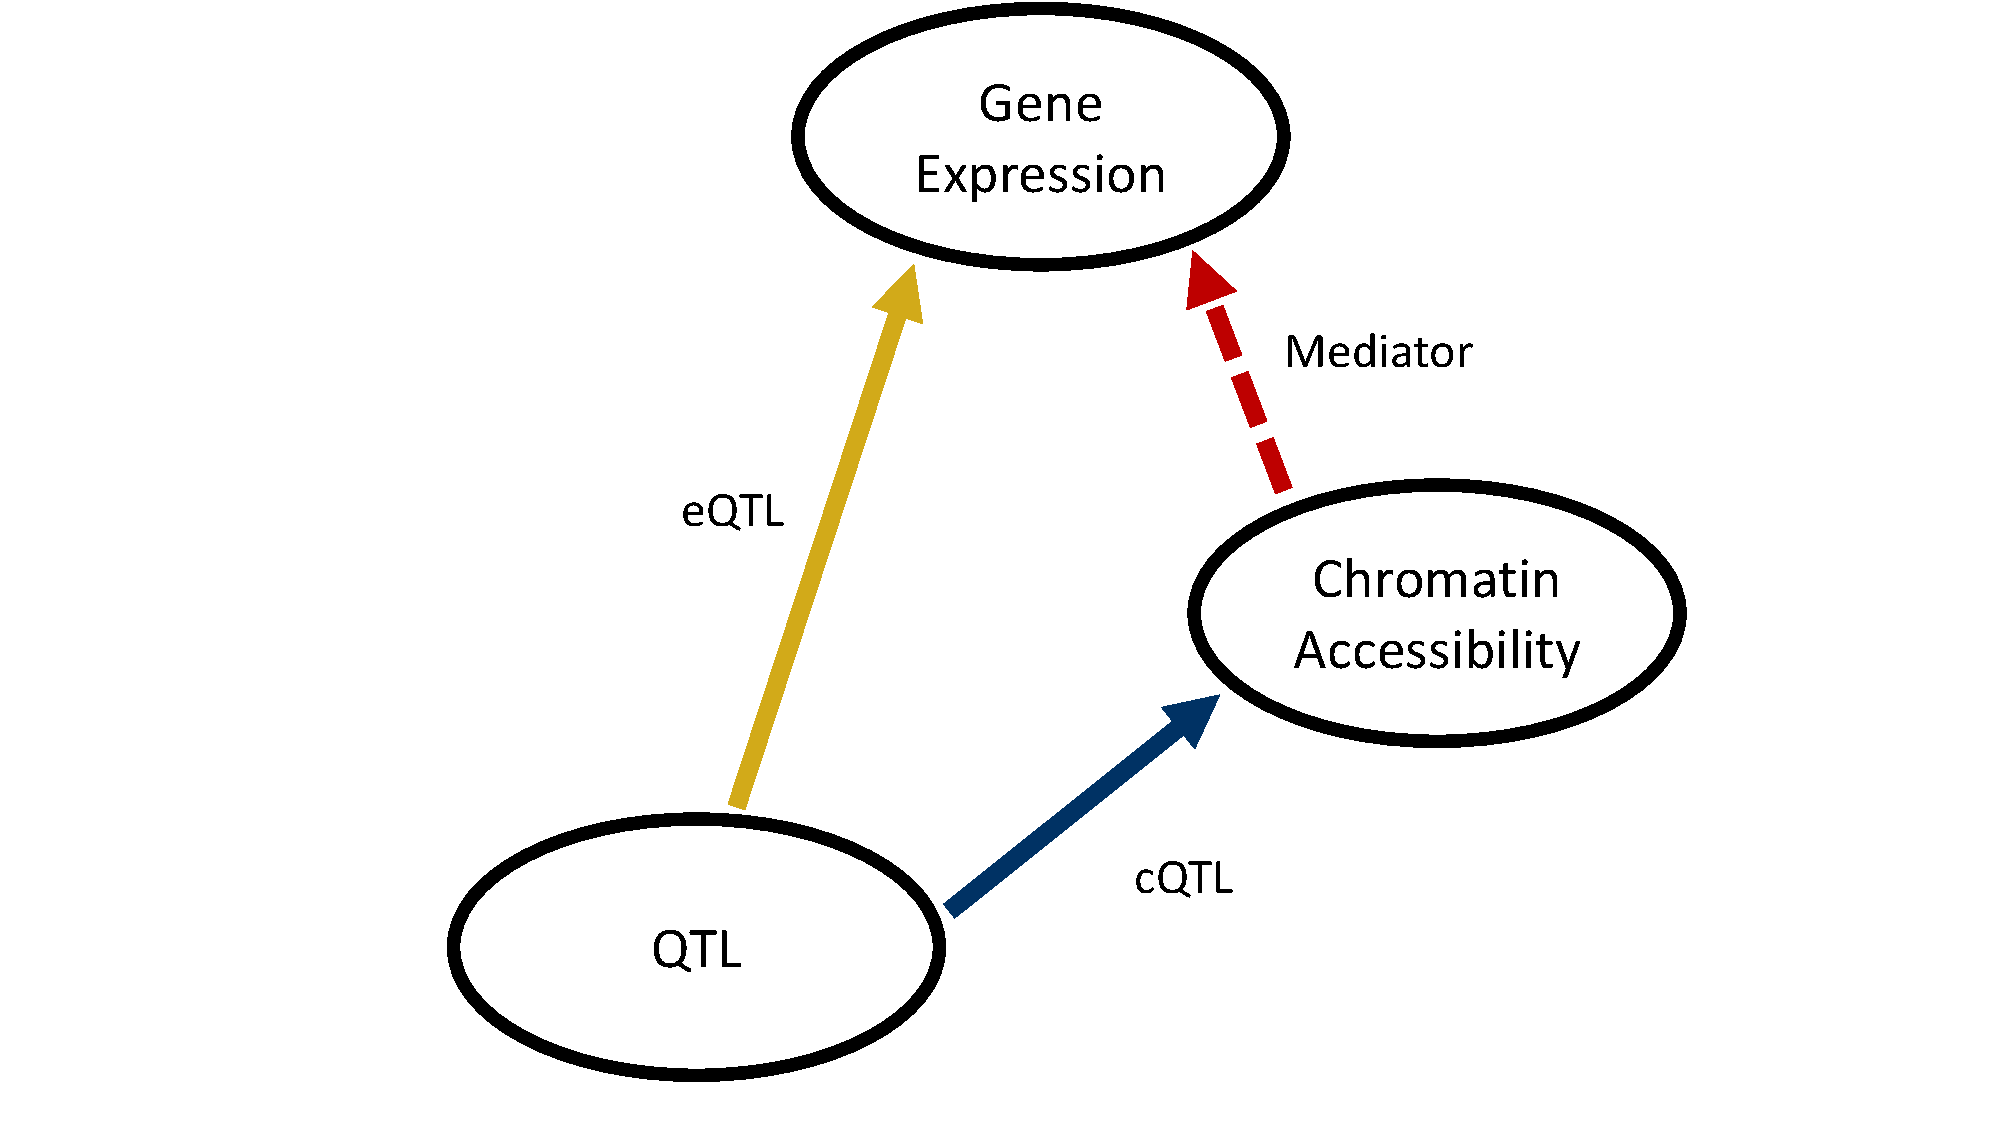
\includegraphics[width=\linewidth, clip, trim={0in 0 0 0in}]{figures/6-mediation/eQTL_cQTL_graph.pdf}
\caption[Simple model for mediation of eQTL effect on gene expression through chromatin accessibility]{The simple relationships being assessed between QTL, chromatin accessibility, and gene expression. The directionality of the relationships between QTL and gene expression and chromatin accessibility is strongly supported in biology, as the haplotype is fixed prior to gene expression and chromatin accessibility dynamics. The assumption of the directionality of the relationship between chromatin accessibility and gene expression is less likely be true in all cases. In reality the relationship may reflect complex equilibriums or be multifactorial and complex. Mediation may also be present and the data are under-powered to detect it. Alternatively, mediation may be present and undetected, because of important additional un-modeled factors, such as the effects of transcription factors and enhancers. \label{fig:graph}}
\end{figure}

\subsection{Genome-wide mediation analysis}

Mediation analysis has previously been used with genomic data \citep{Battle2014,Roytman2018,Wu2018}. Our approach to assessing the statistical support of chromatin state mediating gene expression is similar to the method used by \cite{Chick2016} for detecting mediation of protein abundance through gene expression. We assess evidence for chromatin mediation only in detected genome-wide eQTL because the presence of mediation depends on relationship \ref{rel:eQTL} existing.

We simplify the formal mediation analysis to a genome-wide mediation scan which allows us to detect multiple testing corrected significant mediators following relationships \ref{rel:full_mediator} and \ref{rel:partial_mediator}. Similar to the QTL mapping genome scan described in Eq \ref{eq:alternative_model} and Eq \ref{eq:conditional_model}, the mediation scan involves a comparison of an alternative and a null model at loci across the genome. The alternative model is
\begin{flalign}
f(\text{gene.expression}_{ij}) &= \text{intercept} \\ &+ \text{eQTL}_{i}^{\text{gene} j} + \text{chromatin}_{ik} \nonumber \\ &+ \text{batch}_{i} + \varepsilon_{i}, \nonumber
\label{eq:mediation_alt}
\end{flalign}
and the null model is
\begin{flalign}
f(\text{gene.expression}_{ij}) &= \text{intercept} \\ &+ \text{chromatin}_{ik} \nonumber \\ &+ \text{batch}_{i} + \varepsilon_{i}, \nonumber
\label{eq:mediation_null}
\end{flalign}
where $\text{gene.expression}_{ij}$ is the transcript levels of gene $j$ that has a genome-wide significant eQTL for individual $i$, $\text{eQTL}_{i}^{\text{gene} j}$ is the locus effect for the eQTL of gene $j$, $\text{chromatin}_{ik}$ is the effect of chromatin accessibility at site $k$ for individual $i$, $\text{batch}_{i}$ is the effect of the sequencing center used to sequence the gene expression of individual $i$, and $\varepsilon_{i}$ is the random noise for individual $i$. Whereas with the QTL genome scan the locus effect was changed at each position, for the mediation scan, it is fixed at the eQTL locus, and the chromatin site effect is changed.

Because the eQTL is always included in the alternative model but not the null model, the average mediation logP of the mediation scan should fluctuate around the observed eQTL logP. At chromatin sites where the chromatin accessibility variable contains some or all of the information present in the eQTL founder haplotype states, the mediation logP will drop due to the competition between the eQTL and chromatin terms. Significant drops represent potential sites of full mediation, as in relationship \ref{rel:full_mediator}. Alternatively, jointly fitting the eQTL and chromatin could increase the mediation logP significantly beyond the original eQTL signal. This signal does not correspond exactly to the partial mediation relationship in \ref{rel:partial_mediator}, but similarly represents a site where accounting for chromatin accessibility significantly improves the eQTL signal, which we will refer to as an indirect mediator. 

\subsection{Mediation scan significance thresholds}

Our mediation scan approach allows us to define significance through permutations, similarly to as is done with the QTL scans. EVD can be fit for potential full mediators based on minimum logP from permutation scans, and indirect mediators based on maximum logP. We then use these EVD to produce mediation permP, which can be calculated in terms genome-wide and local chromosome-wide significance, with local in reference to the eQTL, not the gene. Finally we use an FDR procedure to obtain mediation q-values.

\section{Preliminary Results and Discussion}

\subsection{Summaries of the number of associations}

This project is ongoing, and thus the results are preliminary. In fact, results are being re-run as a result of an issue detected from the QTL mapping, which will be discussed further. A breakdown of the numbers of detected eQTL in terms of tissue, local/distal status, and genome-wide/local chromosome-wide significance are in \textbf{Table \ref{tab:eqtl_results}}. Similar summaries for cQTL and mediation are present in \textbf{Tables \ref{tab:cqtl_results}} and \textbf{\ref{tab:mediation_results}}, respectively. 

\subsubsection{eQTL}

We detect more associations in kidney compared to lung and liver, which have similar numbers of associations. These patterns hold true for chromatin accessibility and mediation. For eQTL, we detect genome-wide eQTL for 5-8\% of tested genes across the tissues. In terms of local chromosome-wide significance, the range increases to 17-28\%. The eQTL signal is predominantly local signal, ranging from 74-80\% local, whether genome-wide or local chromosome-wide. 

\subsubsection{cQTL}

We detect more genome-wide associations in chromatin accessibility compared to gene expression, from 13-17\% across the tissues, and similar for local chromosome-wide, 16-28\%. The relative magnitudes for local to distal cQTL are similar to to those in gene expression.  

\subsubsection{Mediation}

We test for mediation in only detected eQTL, and find significant genome-wide evidence ranging from 16-18\% across all tissues for these eQTL. In terms of local chromosome-wide evidence, we see evidence of mediation in 30-43\% of eQTL across all tissues. As with eQTL and cQTL, mediation is appears to be primarily local ranging from 72-82\% and 73-74\% for genome-wide and local chromosome-wide, respectively.

We expect the distal signals to be reduced upon re-processing of the sequence alignments, particularly for cQTL and mediation. Initially reads were included that could align with up to four positions, which resulted in some distal signals, particularly noticeable in the cQTL results. We are currently re-processing to restrict to the reads that align uniquely.

These results show that it is possible to detect eQTL, cQTL, as well as mediation at a genome-wide level in a relatively small sample (47 mice). Considering curves produced by the SPARCC R package from \textbf{Chapter \ref{chap:sparcc}} show that this sample size is not sufficiently powered to detect QTL with effects that explain 50\% of the outcome variation, which suggests that many of these detected QTL have large effects ($> 50\%$). With more CC strains and replicate observations, more eQTL, cQTL, and mediators would be detected.

\begin{table}
\renewcommand{\familydefault}{\sfdefault}\normalfont
\begin{minipage}{\textwidth}
%\captionsetup{width=\textwidth}
\centering
\caption{Number of genes with eQTL detected ($\text{q-value} < 0.1$) in lung, liver, and kidney tissues
\label{tab:eqtl_results}}
\end{minipage}
\begin{minipage}{\textwidth}
\begin{tabularx}{\textwidth}{ll||XXX}
\hline 
& & & \center{Tissue (\%)} & \\
& & Lung & Liver & Kidney \\
\hline\hline
eQTL & genome-wide & 772 (5.3\footnote{Percentage of all tested genes.\label{fn:total_perc}}) & 772 (7.2\footref{fn:total_perc}) & 1092 (8.4\footref{fn:total_perc}) \\
& local chromosome-wide & 2573 (17.8\footref{fn:total_perc}) & 2461 (22.9\footref{fn:total_perc}) & 3680 (28.4\footref{fn:total_perc}) \\
\hline\hline
local-eQTL\footnote{eQTL defined as local if within 10 Mb upstream or downstream of gene TSS.} & genome-wide & 578 (74.9\footnote{Percentage of genes with genome-wide eQTL.\label{fn:gw_eqtl_perc}}) & 597 (77.3\footref{fn:gw_eqtl_perc}) & 881 (80.7\footref{fn:gw_eqtl_perc}) \\
& local chromosome-wide & 1935 (75.2\footnote{Percentage of genes with local chromosome-wide eQTL.\label{fn:cw_eqtl_perc}}) & 1880 (76.4\footref{fn:cw_eqtl_perc}) & 2769 (75.2\footref{fn:cw_eqtl_perc}) \\
\hline
distal-eQTL\footnote{eQTL defined as distal if not within 10 Mb upstream or downstream of gene TSS or on non-local chromosome.} & genome-wide & 203 (26.3\footref{fn:gw_eqtl_perc}) & 183 (23.7\footref{fn:gw_eqtl_perc}) & 223 (20.4\footref{fn:gw_eqtl_perc}) \\
& local chromosome-wide & 638 (24.8\footref{fn:cw_eqtl_perc}) & 581 (23.6\footref{fn:cw_eqtl_perc}) & 911 (24.8\footref{fn:cw_eqtl_perc}) \\
\hline\hline
\end{tabularx}
\end{minipage}
\end{table}

\begin{table}
\renewcommand{\familydefault}{\sfdefault}\normalfont
\begin{minipage}{\textwidth}
%\captionsetup{width=\textwidth}
\centering
\caption{Number of chromatin accessibility sites with cQTL detected ($\text{q-value} < 0.1$) in lung, liver, and kidney tissues
\label{tab:cqtl_results}}
\end{minipage}
\begin{minipage}{\textwidth}
\begin{tabularx}{\textwidth}{ll||XXX}
\hline 
& & & \center{Tissue (\%)} & \\
& & Lung & Liver & Kidney \\
\hline\hline
cQTL & genome-wide & 2150 (14.3\footnote{Percentage of all tested chromatin site.\label{fn:total_perc}}) & 2034 (13.6\footref{fn:total_perc}) & 2589 (17.3\footref{fn:total_perc}) \\
& local chromosome-wide & 2524 (16.8\footref{fn:total_perc}) & 4323 (28.8\footref{fn:total_perc}) & 3351 (22.3\footref{fn:total_perc}) \\
\hline\hline
local-cQTL\footnote{cQTL defined as local if within 10 Mb upstream or downstream of chromatin accessibility site.} & genome-wide & 1802 (83.8\footnote{Percentage of chromatin accessibility sites with genome-wide cQTL.\label{fn:gw_cqtl_perc}}) & 1681 (82.6\footref{fn:gw_cqtl_perc}) & 1982 (76.6\footref{fn:gw_cqtl_perc}) \\
& local chromosome-wide & 2173 (86.1\footnote{Percentage of chromatin accessibility sites with local chromosome-wide cQTL.\label{fn:cw_cqtl_perc}}) & 3376 (78.1\footref{fn:cw_cqtl_perc}) & 2672 (79.7\footref{fn:cw_cqtl_perc}) \\
\hline
distal-cQTL\footnote{cQTL defined as distal if not within 10 Mb upstream or downstream of chromatin accessibility site or on non-local chromosome.} & genome-wide & 409 (19.0\footref{fn:gw_cqtl_perc}) & 388 (19.1\footref{fn:gw_cqtl_perc}) & 688 (26.6\footref{fn:gw_cqtl_perc}) \\
& local chromosome-wide & 351 (13.9\footref{fn:cw_cqtl_perc}) & 947 (21.9\footref{fn:cw_cqtl_perc}) & 679 (20.3\footref{fn:cw_cqtl_perc}) \\
\hline\hline
\end{tabularx}
\end{minipage}
\end{table}

\begin{table}
\renewcommand{\familydefault}{\sfdefault}\normalfont
\begin{minipage}{\textwidth}
%\captionsetup{width=\textwidth}
\centering
\caption{Number of chromatin mediators of gene expression detected ($\text{q-value} < 0.1$) in lung, liver, and kidney tissues
\label{tab:mediation_results}}
\end{minipage}
\begin{minipage}{\textwidth}
%\begin{tabularx}{\textwidth}{ll|c|c|c}
\begin{tabularx}{\textwidth}{ll||XXX}
\hline 
& & & \center{Tissue (\%)} & \\
& & Lung & Liver & Kidney \\
\hline\hline
mediators & genome-wide & 101 (16.5\footnote{Percentage of genome-wide eQTL.\label{fn:total_perc}}) & 117 (18.7\footref{fn:total_perc}) & 170 (18.4\footref{fn:total_perc}) \\
& local chromosome-wide & 188 (30.1\footref{fn:total_perc}) & 273 (43.5\footref{fn:total_perc}) & 380 (41.1\footref{fn:total_perc}) \\
\hline\hline
local-mediators\footnote{Mediators defined as local if within 10 Mb upstream or downstream of eQTL.\label{fn:local_mediator}} & genome-wide & 73 (72.3\footnote{Percentage of genome-wide mediators.\label{fn:gw_mediator_perc}}) & 96 (82.1\footref{fn:gw_mediator_perc}) & 140 (82.4\footref{fn:gw_mediator_perc}) \\
& local chromosome-wide & 139 (73.9\footnote{Percentage of local chromosome-wide mediators.\label{fn:cw_mediator_perc}}) & 204 (74.7\footref{fn:cw_mediator_perc}) & 282 (74.2\footref{fn:cw_mediator_perc}) \\
\hline
distal-mediators\footnote{Mediator defined as distal if not within 10 Mb upstream or downstream of eQTL or on non-local chromosome.\label{fn:distal_mediator}} & genome-wide & 28 (27.7\footref{fn:gw_mediator_perc}) & 21 (17.9\footref{fn:gw_mediator_perc}) & 30 (17.6\footref{fn:gw_mediator_perc}) \\
& local chromosome-wide & 49 (26.1\footref{fn:cw_mediator_perc}) & 69 (25.3\footref{fn:cw_mediator_perc}) & 98 (25.8\footref{fn:cw_mediator_perc}) \\
\hline
local-mediators\footref{fn:local_mediator} of local-eQTL\footnote{eQTL defined as local if within 10 Mb upstream or downstream of gene TSS.} & genome-wide & 70 (69.3\footref{fn:gw_mediator_perc}) & 92 (78.6\footref{fn:gw_mediator_perc}) & 138 (81.2\footref{fn:gw_mediator_perc}) \\
& local chromosome-wide & 129 (68.6\footref{fn:cw_mediator_perc}) & 185 (67.8\footref{fn:cw_mediator_perc}) & 270 (71.1\footref{fn:cw_mediator_perc}) \\
local-mediators\footref{fn:local_mediator} of distal-eQTL\footnote{eQTL defined as distal if not within 10 Mb upstream or downstream of gene TSS or on non-local chromosome.} & genome-wide & 3 (3.0\footref{fn:gw_mediator_perc}) & 4 (3.4\footref{fn:gw_mediator_perc}) & 2 (1.2\footref{fn:gw_mediator_perc}) \\
& local chromosome-wide & 10 (5.3\footref{fn:cw_mediator_perc}) & 19 (7.0\footref{fn:cw_mediator_perc}) & 12 (3.2\footref{fn:cw_mediator_perc}) \\
\hline\hline
\end{tabularx}
\end{minipage}
\end{table}

\subsection{eQTL and cQTL mapping results}

As shown in \textbf{Tables \ref{tab:eqtl_results}} and \textbf{\ref{tab:cqtl_results}} most QTL for expression and chromatin accessibility are local, as can be seen in \textbf{Figure \ref{fig:grid_plot}} as the band along the diagonal of the grids. There are QTL on the off-diagonal, representing distal-QTL. There is some evidence of vertical bands in the cQTL, which would represent a region of the genome that regulates the chromatin accessibility at many sites. It is likely that many of these bands will disappear once reads are restricted to those that uniquely align.

\begin{figure}
\renewcommand{\familydefault}{\sfdefault}\normalfont
\centering
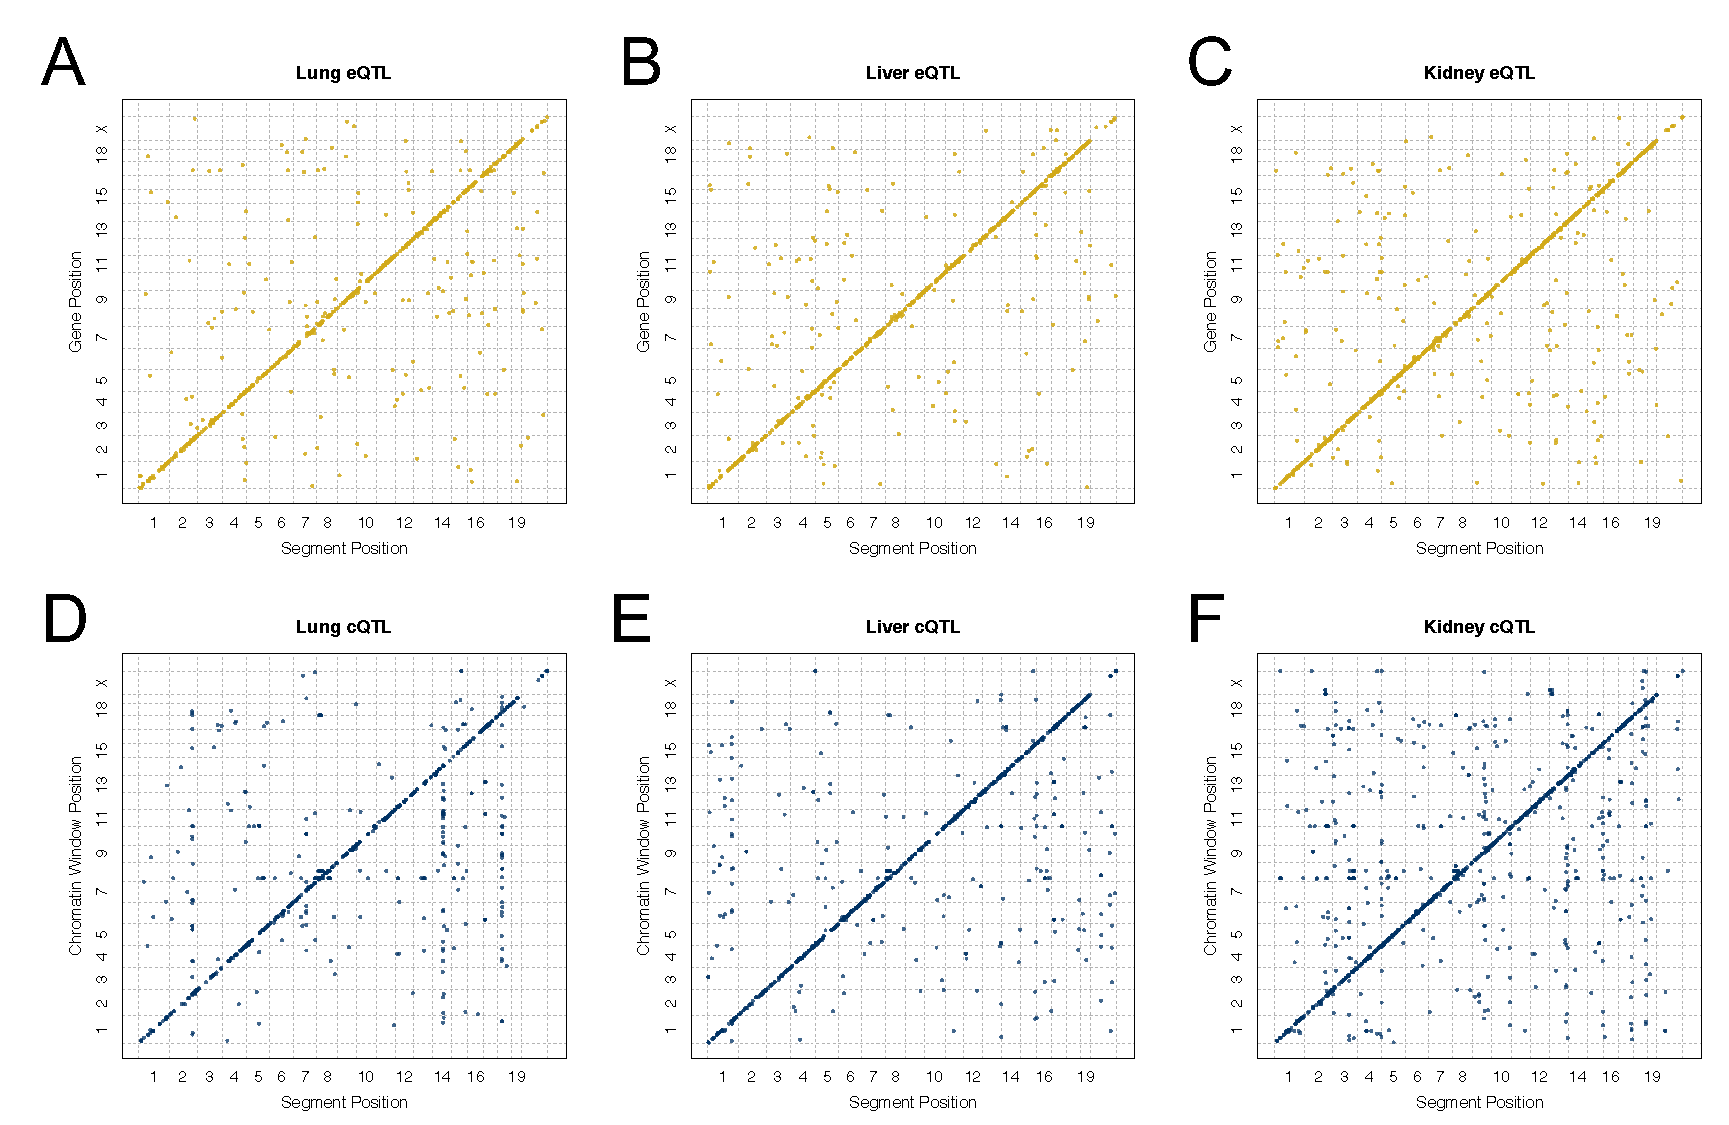
\includegraphics[width=\textwidth, trim={0in 0in 0in 0in}, clip]{figures/6-mediation/all_qtl_maps.pdf}
\caption[eQTL and cQTL signals for lung, liver, and kidney]{Grid plots of eQTL (yellow) and cQTL (blue) in lung (A,D), liver (B,E) , and kidney (C,F), significant at q-value $\le 0.1$. There is a predominance of local-eQTL and local-cQTL relative to distal signals, matching the biological expectation. \label{fig:grid_plot}}
\end{figure}

\subsection{Mediation results}

As shown in \textbf{Tables \ref{tab:mediation_results}}, we do see instances of strong evidence of chromatin accessibility at genomic positions mediating the effect of an eQTL on gene expression. Although it is not possible to prove causality with these data, it is consistent with biological expectation were the eQTL to be functionally active through chromatin accessibility. A strong example of mediation of the expression of the gene \textit{Dynltb1} in lung tissue through local chromatin accessibility is provided in \textbf{Figure \ref{fig:mediation_example}}. This example also highlights an observation that cQTL tend to have larger effects than eQTL, suggesting that there is some buffering of the effect on expression. This is consistent or parallel with a similar dynamic seen in comparison of eQTL effects being larger than pQTL in \cite{Battle2015}. We will discuss a systematic approach to checking this QTL effect buffering later on in the Discussion.

\begin{figure}
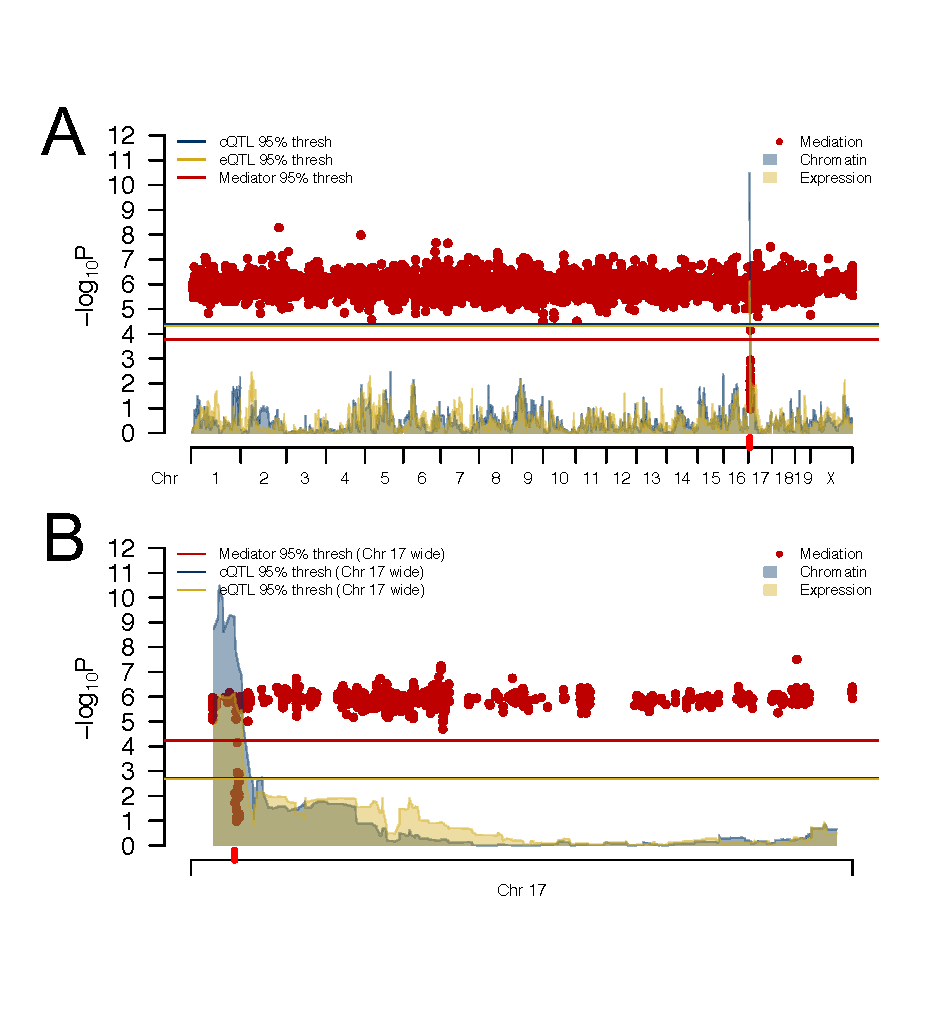
\includegraphics[width=\textwidth, trim={0in 0.2in 0in 0in}, clip]{figures/6-mediation/mediation_example.pdf}
\caption[Example of evidence consistent with chromatin accessibility mediating between eQTL and gene expression]{Genome scans for expression levels (yellow), chromatin accessibility (blue) and chromatin mediation (red) of \textit{Dynltb1}, a gene located on chromosome 17, in 47 CC lines in lung tissue. There is both a strong local-eQTL and a strong local-cQTL present near the transcription start site of \textit{Dynltb1} (red tick). The steep logP drop in the mediation scan at or near the co-localizing QTL is supportive of mediation of \textit{Dynltb1} expression through local chromatin accessibility. Genome-wide scan with corresponding significance thresholds (A). Scan of chromosome 17, the local chromosome, with corresponding local chromosome-wide significance thresholds (B). \label{fig:mediation_example}}
\end{figure}

\subsubsection{Identifying co-localizing eQTL and cQTL with mediation and without}

Statistical detection of mediation does not simply reflect that eQTL and cQTL are located physically nearby; in fact, eQTL and cQTL can have the same position and not provide any evidence of mediation. The formal mediation involves a statistical test in which the mediator, chromatin accessibility, must absorb much of the effect of the detected eQTL for mediation to be detected. eQTL and cQTL could co-localize, but have highly different founder haplotypes driving the effects. We find that using the regressions coefficients as founder allele effects can visually distinguish co-localizing eQTL and cQTL with mediation and co-localizing eQTL and cQTL without mediation, and even quantified with Spearman's correlation, as in \textbf{Figure \ref{fig:colocalization}}. In the case of mediation, the allele effects of eQTL for \textit{Gm14403} are highly correlated with the allele effects of the co-localizing cQTL. In the case of no mediation, as in \textit{Ear2}, the correlation is much lower between effect vectors. 

\begin{figure}
\renewcommand{\familydefault}{\sfdefault}\normalfont
\centering
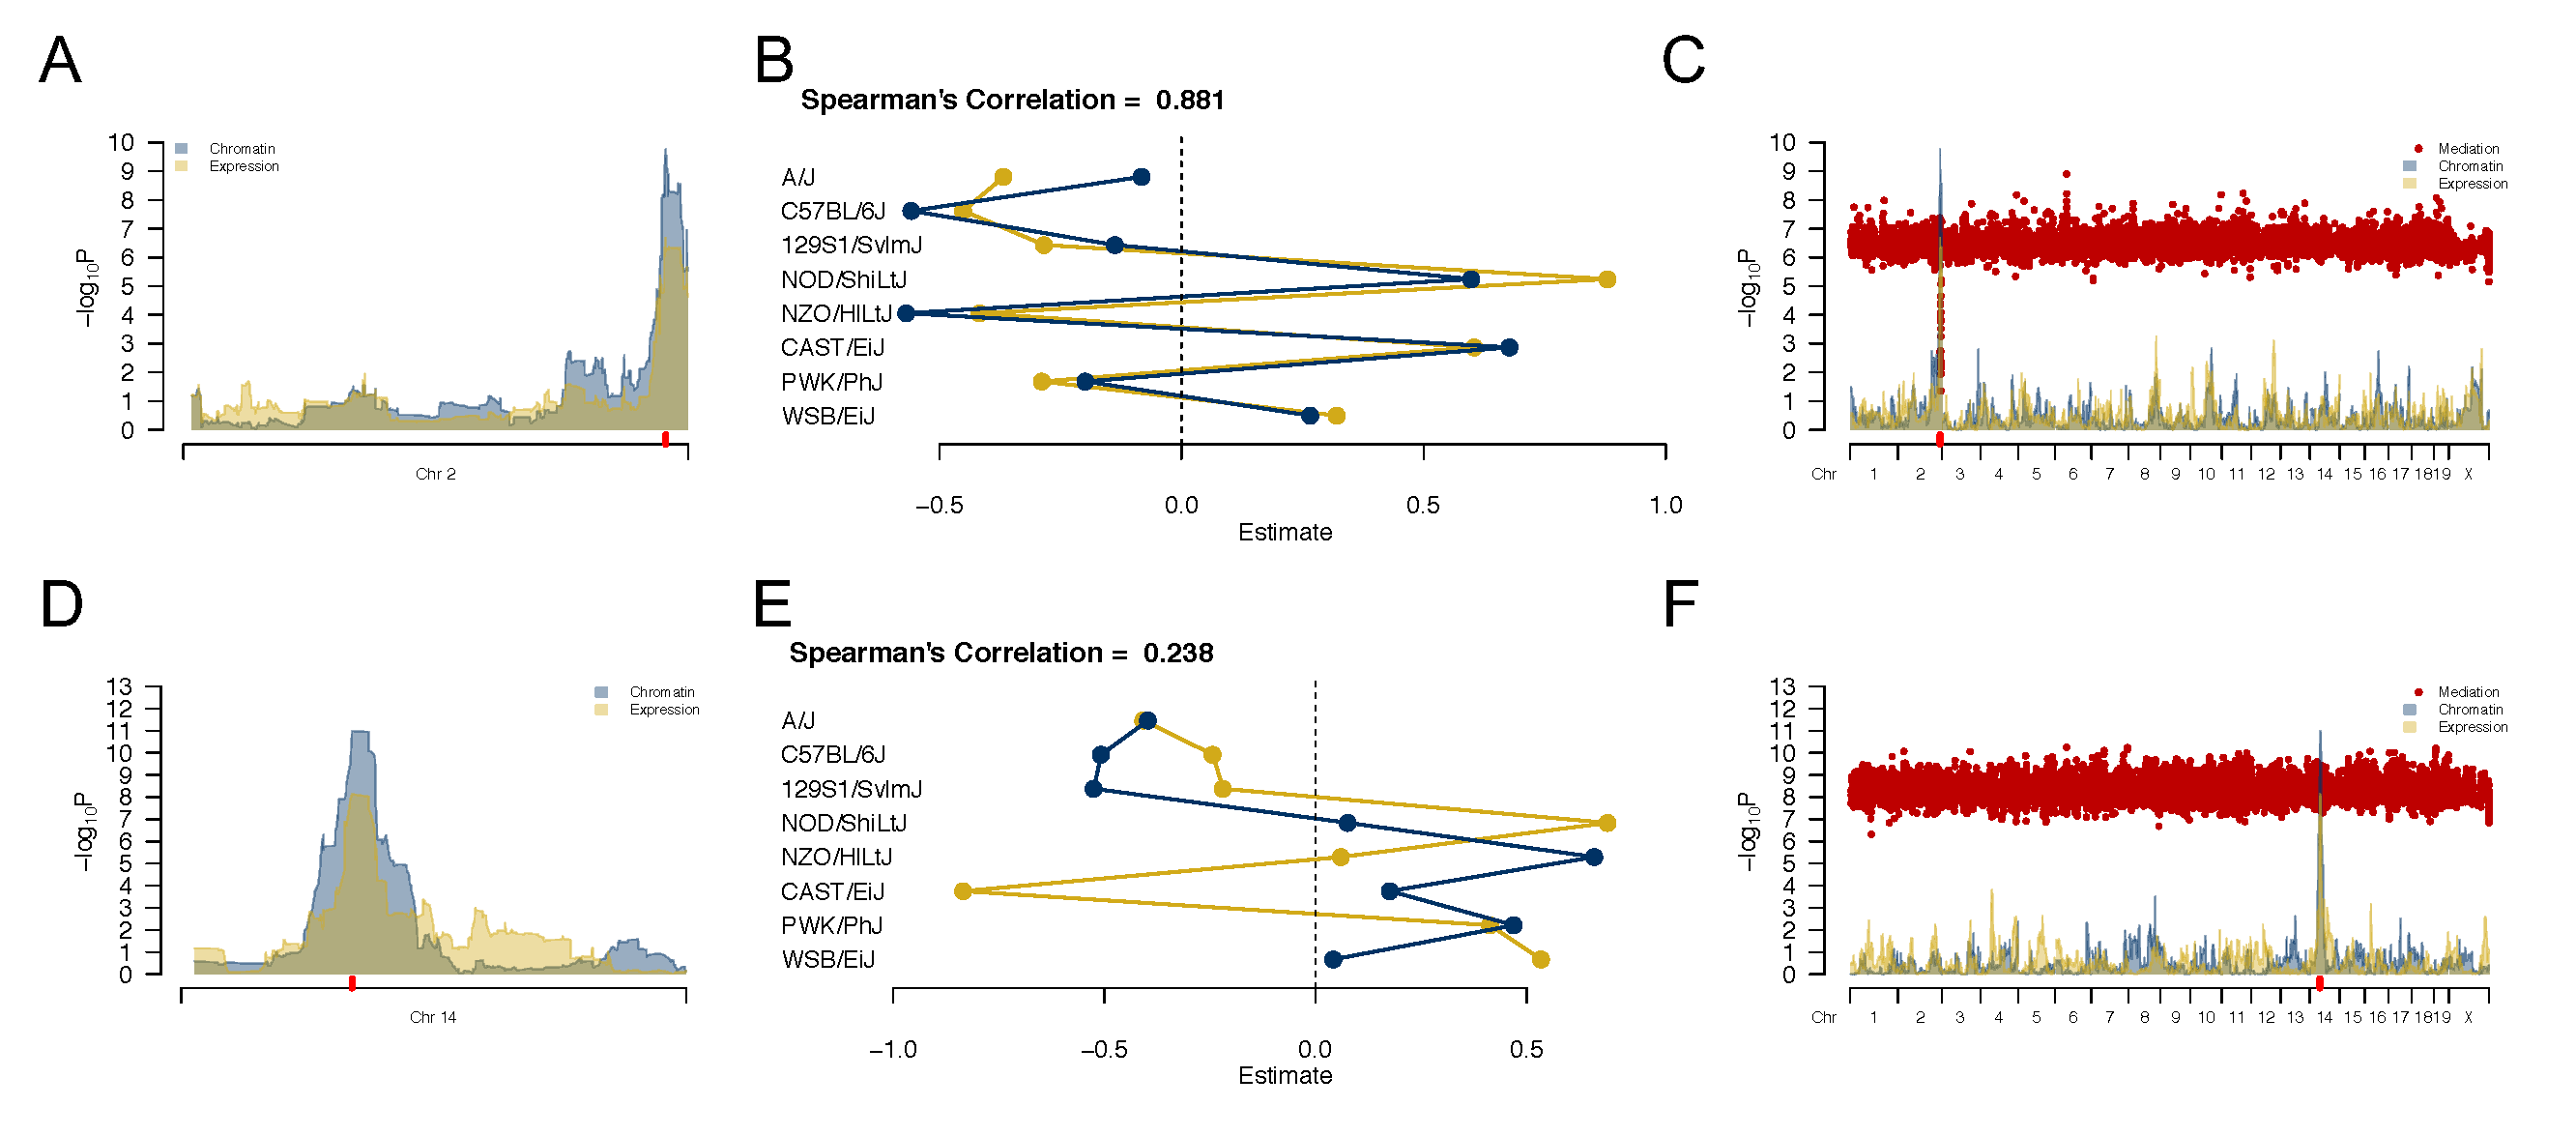
\includegraphics[width=\textwidth]{figures/6-mediation/mediator_or_colocal.pdf}
\caption[Co-localizing eQTL and cQTL not sufficient for mediation]{Co-localizing eQTL and cQTL are not sufficient for mediation. Co-localizing QTL are observed for which there is evidence of mediation for the gene \textit{Gm14403} in lung tissue (A). The haplotype effects at the eQTL and cQTL position (red tick) are highly correlated (B). The resulting mediation scan shows strong evidence of mediation (C). For the gene \textit{Ear2} in lung, co-localizing eQTL and cQTL are also observed (D). The eQTL and cQTL haplotype effects do not correlate closely, with a particularly strong CAST effect in expression but not in chromatin (E). A mediation signal is not detected for \textit{Ear2}.\label{fig:colocalization}}
\end{figure}

\subsubsection{eQTL, cQTL, and mediation are highly local}

As presented in \textbf{Tables \ref{tab:eqtl_results}}, \textbf{\ref{tab:cqtl_results}}, and \textbf{\ref{tab:mediation_results}}, the QTL and mediators are largely local. We present all three levels of signals simultaneously through radial plots for each tissue in \textbf{Figure \ref{fig:circos_plot}}. The plots contain a lot of information, but we emphasize that the inner circles have colored lines connecting eQTL to gene TSS (yellow), cQTL to chromosome accessibility region (blue), and mediator to eQTL (red). Local signals present as a line segment or stick, whereas distal signals are curved lines that connect positions on the circle. Overwhelmingly, the inner circle is covered in line segments representing local signals. In particular, the presence of red local mediators predominantly occur where both local eQTL and cQTL are present. We do not formally require this in our genome-wide mediation test, though the co-occurrence supports that we are detecting true signals.

\subsubsection{Detection of alignment issue in chromatin accessibility data}

In \textbf{Figure \ref{fig:circos_plot}}, a strong set of distal cQTL are present in \textbf{Figures \ref{fig:circos_plot}A} and \textbf{\ref{fig:circos_plot}C}, representing cQTL on chromosome 8 for chromatin accessibility regions on chromosome 18. Further investigation revealed that the chromosome 18 chromatin outcomes had a strong WSB signal, matching the haplotype pattern present in the region on chromosome 8. This pattern of effects would correspond to true distal-cQTL, though it also raised the possibility that the sequence similarity in the regions are resulting in reads from chromosome 8 aligning to chromosome 18. To reduce the risk of false distal QTL and mediators, we are re-processing the data to only use reads that uniquely align within the genome.

\begin{figure}
\renewcommand{\familydefault}{\sfdefault}\normalfont
\centering
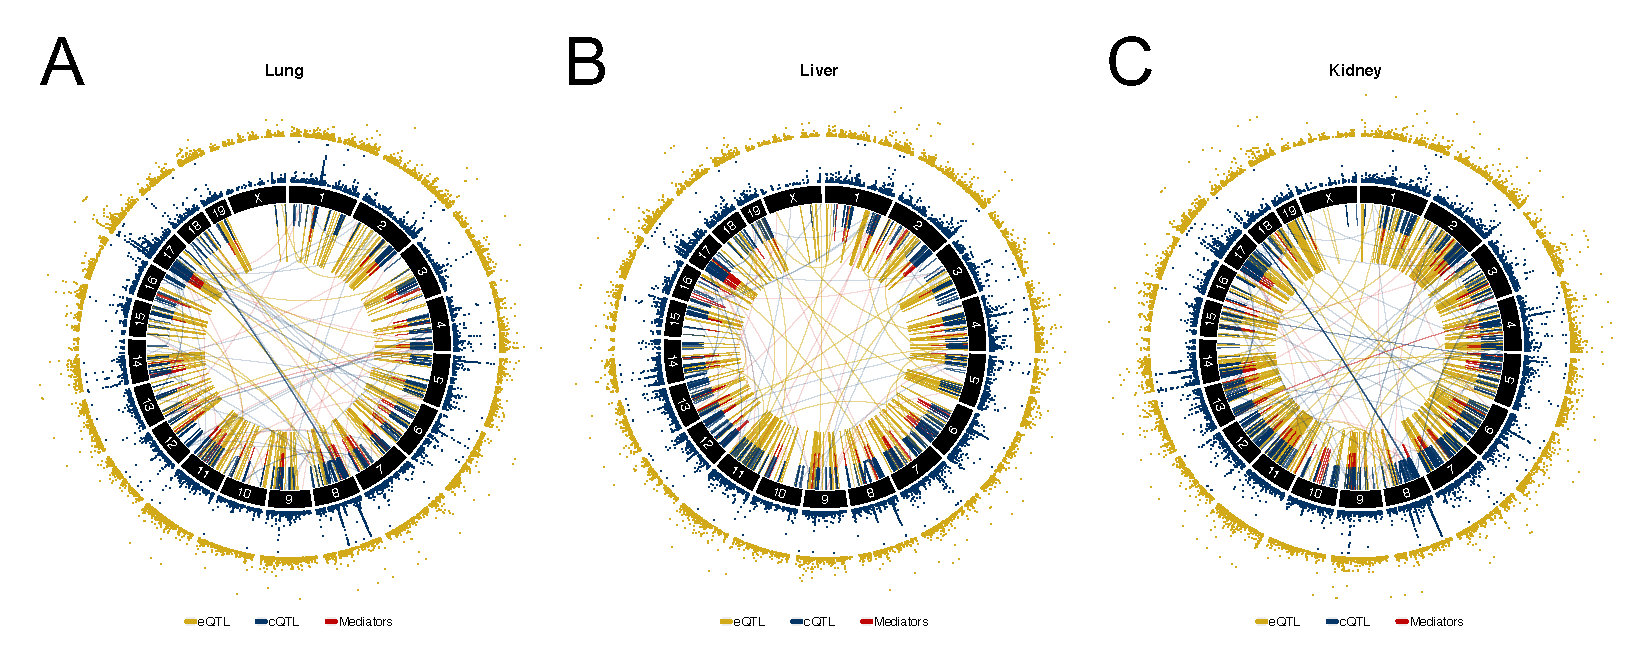
\includegraphics[width=\textwidth]{figures/6-mediation/all_circos.pdf}
\caption[eQTL, cQTL, and mediation signal is primarily local in lung, liver, and kidney]{Radial plots of eQTL (yellow), cQTL (blue), and mediation (red) in (A) lung, (B) liver, and (C) kidney. The outer-most yellow ring depicts the local-eQTL permP and the middle blue ring is the local-cQTL permP. The inner circle has lines connecting gene TSS to eQTL (yellow), chromatin accessibility sites to cQTL (blue), and eQTL to mediating chromatin accessibility sites (red), each representing a significant signal of q-value $\le 0.01$. There is a predominance of local-eQTL, local-cQTL, and local-mediators compared to distal signals. Mediation signals primarily occur where both eQTL and cQTL are detected.
\label{fig:circos_plot}}
\end{figure}

\subsection{Distance from QTL or mediator to outcome}

We investigated the relationship between statistical association and physical distance from gene TSS for putative eQTL, chromatin accessibility region for putative cQTL, and eQTL for putative mediator, for signals on the local chromosome. We see that putative QTL or putative mediators nearby their outcome tend to have more statistically significant associations, which corresponds to the predominance of local signal. We present genome-wide significant results in \textbf{Figure \ref{fig:genomewide_dist}} and local chromosome-wide significant in \textbf{Figure \ref{fig:chrwide_dist}}. We also observe an odd pile up in cQTL with small p-values around 50 Mb away from the chromatin outcome in lung and kidney, likely representing distal bands occurring due to the alignment issue. We expect these to disappear after the data are re-processed.

\begin{figure}
\renewcommand{\familydefault}{\sfdefault}\normalfont
\centering
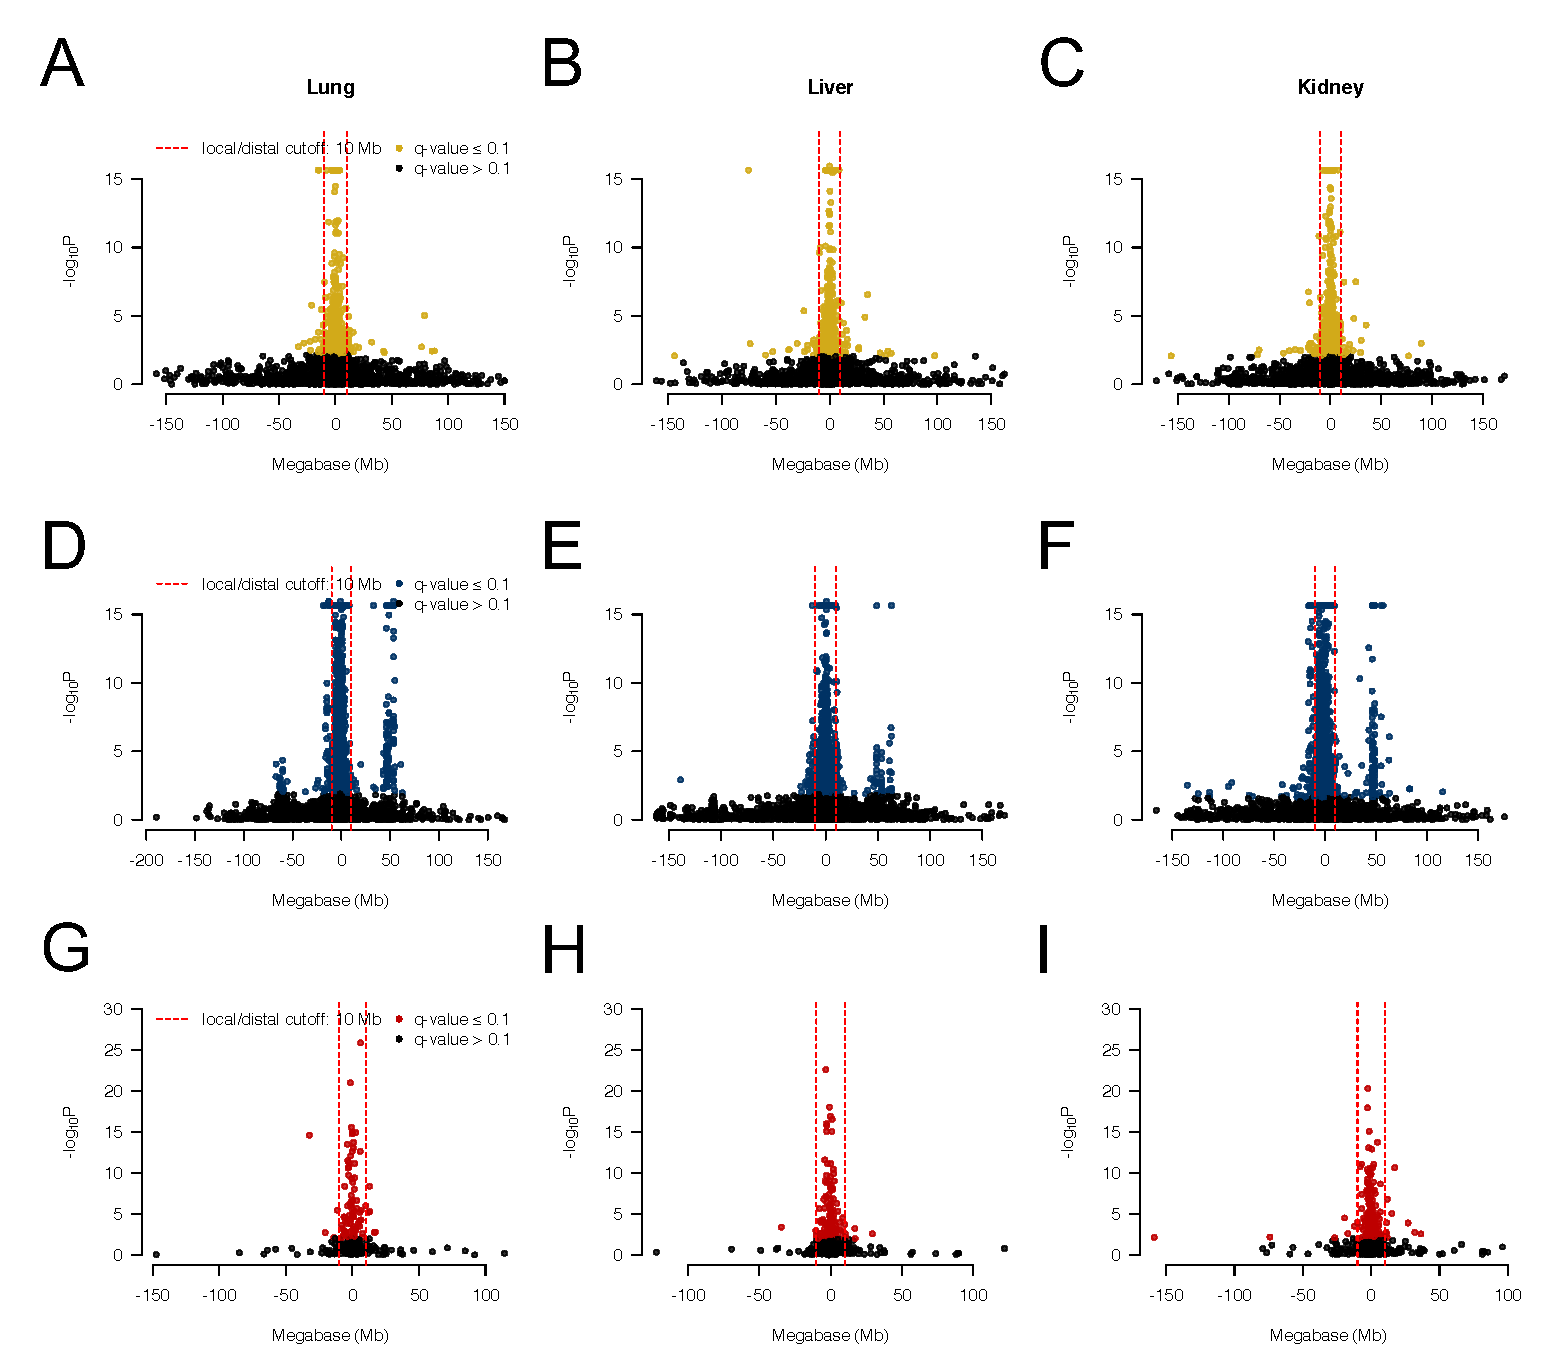
\includegraphics[width=\textwidth]{figures/6-mediation/genome_wide_dist.pdf}
\caption[Genome-wide association signal increases as distance decreases from gene, chromatin region, and eQTL]{The genome-wide permP for eQTL (A-C), cQTL (D-F), and mediators (G-I) by distance (Mb) from gene TSS, chromatin site, and eQTL, respectively. Associations that do not present on the local-chromosome are not shown. The red dashed lines represent 10 Mb upstream and downstream of gene TSS, chromatin site, or eQTL for classifying an association as local or distal. Significant signals (colored symbols), based on $\text{q-value} \le 0.1$, are largely local. cQTL exhibit an interesting pattern of non-syntenic association on the local chromosome, clustering around 50 Mb from the chromatin site. This pattern is observed in all tissues, but is more pronounced in lung and kidney (\textbf{Figures \ref{fig:genomewide_dist}D} and \textbf{\ref{fig:genomewide_dist}E}). The figures for the chromosome-wide results are present in \textbf{Figure \ref{fig:chrwide_dist}}.\label{fig:genomewide_dist}}
\end{figure}

\begin{figure}
\renewcommand{\familydefault}{\sfdefault}\normalfont
\centering
\includegraphics[width=\textwidth]{figures/6-mediation/chrom_wide_dist.pdf}
\caption[Local chromosome-wide association signal increases as distance decreases from gene, chromatin region, and eQTL]{The local chromosome-wide permP for eQTL (A-C), cQTL (D-F), and mediators (G-I) by distance (Mb) from gene TSS, chromatin site, and eQTL, respectively. Associations that do not present on the local-chromosome are not shown. The red dashed lines represent 10 Mb upstream and downstream of gene TSS, chromatin site, or eQTL for classifying an association as local or distal. Significant signals (colored symbols), based on $\text{q-value} \le 0.1$, are largely local. cQTL exhibit the same interesting pattern of non-syntenic association on the local chromosome as seen in the genome-wide results, clustering around 50 Mb from the chromatin site. We see more local signals are identified through a local chromosome test, though the number of non-local associations (based on 10 Mb) on the local chromosome also increase. The figures for the genome-wide results are present in \textbf{Figure \ref{fig:genomewide_dist}}.
\label{fig:chrwide_dist}}
\end{figure}

\subsection{Buffering of eQTL effect from cQTL effect}

Visually we see evidence that the cQTL effects are more extreme than the eQTL effects based on the magnitudes of the associations at the QTL in \textbf{Figures \ref{fig:mediation_example}} and \textbf{\ref{fig:colocalization}}. This dynamic is consistent with biology in that gene expression is further down the regulatory pathway of transcription, and thus more steps for noise to be introduced into the system. It is also similar to findings in \cite{Battle2015} on the effect of eQTL on gene expression in comparison to the effect of pQTL on protein abundance. Prior to publication, we plan to systematically assess this dynamic. \cite{Battle2015} uses human data and thus models QTL based on SNP genotypes, thus the QTL effect likely represents a scalar estimate of the effect of a dose of the minor allele of the SNP. With haplotype-based association in the CC, we instead estimate an eight element vector as an effect, making it non-trivial to estimate a similar quantity. We plan to use a regression approach in which the regression coefficients, call them $\bbeta$ from the $\text{QTL}_{i}$ term in Eq \ref{eq:alternative_model} is constrained through the imposition of a variance component: $\bbeta \sim \text{N}(\bzero, \bI \tausq)$ \citep{Wei2016}. $\tausq$, the variance component, is a scalar summary of the QTL effect, with larger variance components corresponding to larger effects.  At all eQTL and cQTL, we can estimate $\widehat{\tausq}_{\text{cQTL}}$ and $\widehat{\tausq}_{\text{eQTL}}$ and summarize the overall distributions in comparison to each other. We can also look specifically at cQTL and eQTL that likely represent mediation pairs. Finally, we can look at effects sizes based on local and distal status. Random effect fits of the locus effect are computationally expensive, therefore not appealing for mapping scans with cQTL and eQTL. However, with the set of tests constrained to only the detected cQTL and eQTL, it is feasible.

\subsection{Frequency of distal-QTL signal in comparison to local-QTL}

\cite{Battle2014} identified local-eQTL in 78.8\% and distal-eQTL in 2.9\% of all the genes tested. In kidney, for which we detected the most QTL, we detect local eQTL in 6.8\% and distal eQTL in 1.7\% of tested genes. The disparity is almost certainly the result of the data comprising 47 individuals in comparison to 922. More CC strains and replicate observations would increase power to detect the QTL, and likely mediation as well. The relative proportions between local and distal QTL are also closer in the CC mice than human data. Some of the distal-QTL will likely disappear once the data are re-processed, particularly in the cQTL. There is also the potential that a small sample of 47 CC mice are slightly prone to false positive distal QTL in comparison to 922 humans. Haplotype-based association fits a comparatively complex model in comparison to SNP genotypes, and though the CC have fairly good balance in founder haplotype contributions, there are deviations from it at certain loci. This can result in situations in which a single or a few individuals has a rare founder allele at a locus and an extreme phenotype, resulting in a sudden association (discussed in \textbf{Chapter \ref{chap:mi}}). Shrinkage approaches could account for this, and would certainly reduce distal-QTL in comparison to local-QTL, but would prove computationally challenging. More CC strains and replicate observations would respectively result in more balanced founder contributions within the sample and reduction in outliers that power false associations.

There is value in the amount of local-QTL signal that we are able to detect given the sample size, and particularly that there is evidence of mediation at some of the eQTL. Our use of local chromosome-wide significance also supports our ability to detect local-QTL, as the proportion of local-eQTL out of all genes increases to 21.4\% from 6.8\% compared to 7\% from 1.7\% for distal-eQTL in kidney tissue,  suggesting that predominantly more local-eQTL, and thus likely real signal is being detected.

\subsection{Complexity of the underlying mediation}

We use a simplistic model for the mediation of the eQTL effect (\textbf{Figure \ref{fig:graph}}). It is likely that the true relationship between gene expression and chromatin accessibility is complex and multifactorial for many genes. A simplistic mediation model as well as potential heterogeneity in the data with respect to un-modeled factors would greatly reduce power to detect mediation. We present these results not as definitive catalogue of genes with expression that is modulated by chromatin accessibility, but rather as proof of principle that simplistic mediation models can be used to detect strong signals, even in small samples. Another approach to consider would be to extract the variants contained within the genomic intervals from the ISVdb resource \citep{Oreper2017}, and more complex mediation models could be explored.

\subsection{Summary}

In this study, we map eQTL and cQTL in lung, liver, and kidney tissues in 47 male CC mice, using a multi-stage conditional fitting approach, which allows for the detection of multiple QTL per outcome. We detect mediation of the eQTL effect on gene expression through chromatin accessibility. We find that signals for QTL and mediation are predominantly local. We note that this is a small sample of CC mice with only a single observation per strain, and is thus only powered to detect QTL with very large effects. cQTL effects appear to be larger than eQTL effects, and we describe a novel approach for quantifying this for a multiparental population like the CC. The ISVdb resource could also be used to further investigate the relationships underlying eQTL and potentially mediating cQTL. This study demonstrates that the CC can be a powerful resource for integrative experiments, which largely remains untapped.

\newpage

\section{Additional Figures}

\begin{figure}[h!]
\renewcommand{\familydefault}{\sfdefault}\normalfont
\centering
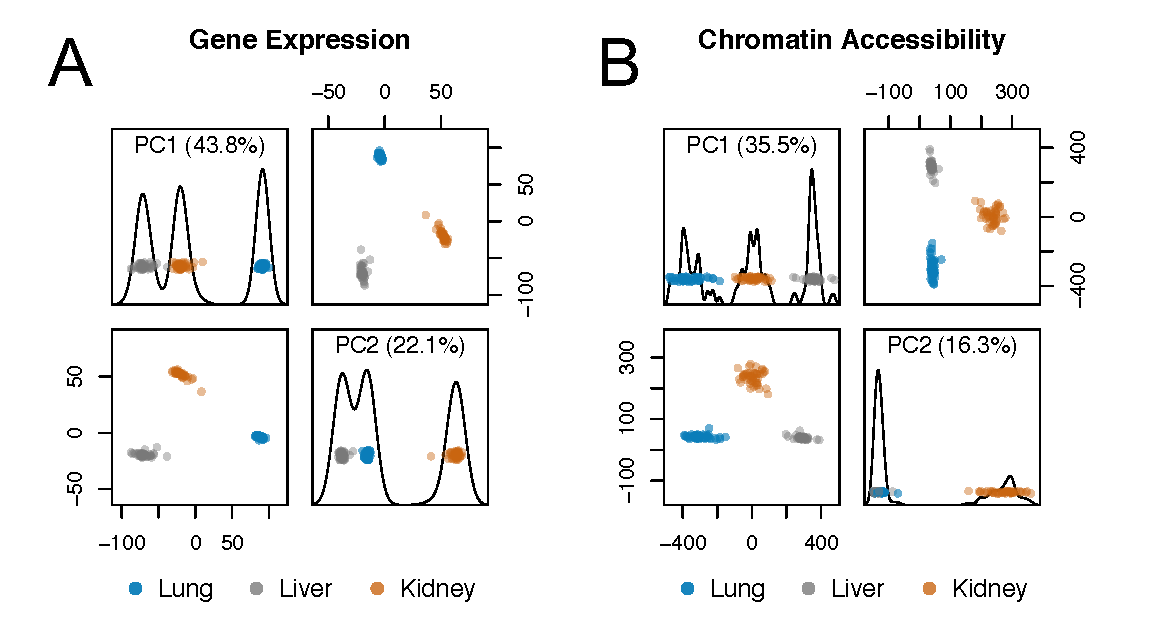
\includegraphics[width=\textwidth, trim={0in 0in 0in 0in}, clip]{figures/6-mediation/pca_processed.pdf}
\caption[Principal components of gene expression and chromatin accessibility]{Principal components (PC) analysis of gene expression (A) and chromatin accessibility (B) for lung (blue), liver (gray), and kidney (orange) tissue samples derived from RNA-Seq and ATAC-Seq data, respectively. PC 1 and 2 capture a majority of the variance and show a greater amount of between tissue variability than within tissue variability. \label{fig:pca_plots}}
\end{figure}





